\section{Background}

\subsection{UPPAAL}
UPPAAL \cite{Larsen1997} is a complete tool for modeling, simulation, and verification of real-time systems. Systems can be modeled as networks of automata and timed automata. A system is composed of one or more models that consist of locations and transitions between locations. Simulation involves traversing the state space to obtain possible paths within the defined system. Simulation is used to interactively check if the system behaves as expected. Verification is realized through model-checking. In the process of verification, properties defined for the system are determined to be valid or not. If the property is found to be false, UPPAAL will produce a diagnostic trace, a path through the system that contradicts the checked property. 

UPPAAL is an appropriate tool to model a robot swarm. A robot swarm is composed of multiple uniform robots. A single robot can be modeled as a timed automaton implementing an algorithm of our choice. A system consisting of multiple uniform timed automata can be used to simulate an algorithm implementation for a robot swarm. This allows us to simulate the robot swarm and perform verification. Verification through model checking can be utilized to verify the correctness of the implementation of the algorithm as well as for the emergence of the desired behavior of the swarm.


\subsection{Timed automata in UPPAAL}
The timed automaton defined in the work of Rajeev Alur and David Dill \cite{Alur1990} is a basis for timed automata used in UPPAAL. Additionally, UPPAAL extends the Definition \ref{def:automaton} of the automaton with invariants and variables of boolean and integer type. The invariant is a progression condition on the system. It states that the system is allowed to stay in a given location only for a specified time before being forced to transition. A transition between locations can be decorated with a guard, a logical condition on the system variables, or clocks. If the logical value of the guard is true, the transition is enabled and disabled otherwise. Transitions can be associated with the synchronization action. Synchronization in UPPAAL is based on handshaking; therefore, one transition is responsible for sending the synchronization signal, and one or more transitions will wait for it. A transition that is waiting for the synchronization signal will remain disabled until the signal is received. This mechanism allows for multiple processes to synchronize their transitions. During transition, it is possible to reset clocks and assign values to variables. These clock and variable values are then used to determine the logical value of the transition guards.

\newpage
\begin{definition}[Definition of timed automaton \cite{Alur1990}]
A timed automaton is a tuple $(\Sigma, S, S_0, C, E)$ where:\\
$\Sigma$ - input alphabet;\\
$S$ - finite set of automaton states;\\
$S_0 \subseteq S$ - set of start states; \\
$C$ - finite set of clocks; \\
$E \subseteq S \times S [\Sigma \cup {\epsilon}] \times 2^C \times \Phi(C)$ - set of transitions\\\\
An edge in timed automaton is a tuple $\langle s, s', \sigma, \lambda \delta \rangle$, where:\\
$s$ - origin state;\\
$s`$ - destination state;\\
$\sigma$ - input symbol for the transition;\\
$\lambda$ - set of clocks to be reset with this transition;\\
$\delta$ - condition enabling the transition;\\
\label{def:automaton}
\end{definition}


\subsection{Modeling in UPPAAL}


% Pseudo-code for mutex
\begin{figure}[H]
\caption{Peterson’s mutual exclusion algorithm 
\label{fig:mutex_code}
\cite{SmallTutorial2009}, \cite{Peterson1981}}
\begin{tabular}{|p{0.5\textwidth}|p{0.5\textwidth}|}
\hline
\textbf{Process 1} & \textbf{Process 2} \\
\hline
\begin{lstlisting}[basicstyle=\ttfamily]
req1=1;
turn=2;
while(turn!=1 && req2!=0);
// critical section:
job1();
req1=0;
\end{lstlisting}
&
\begin{lstlisting}[basicstyle=\ttfamily]
req2=1;
turn=1;
while(turn!=2 && req1!=0);
// critical section:
job2();
req2=0;
\end{lstlisting}
\\
\hline
\end{tabular}
\end{figure}


% Mutex implementation in UPPAAL
\begin{figure}[H]
\caption{Mutex automata in UPPAAL \cite{SmallTutorial2009}}
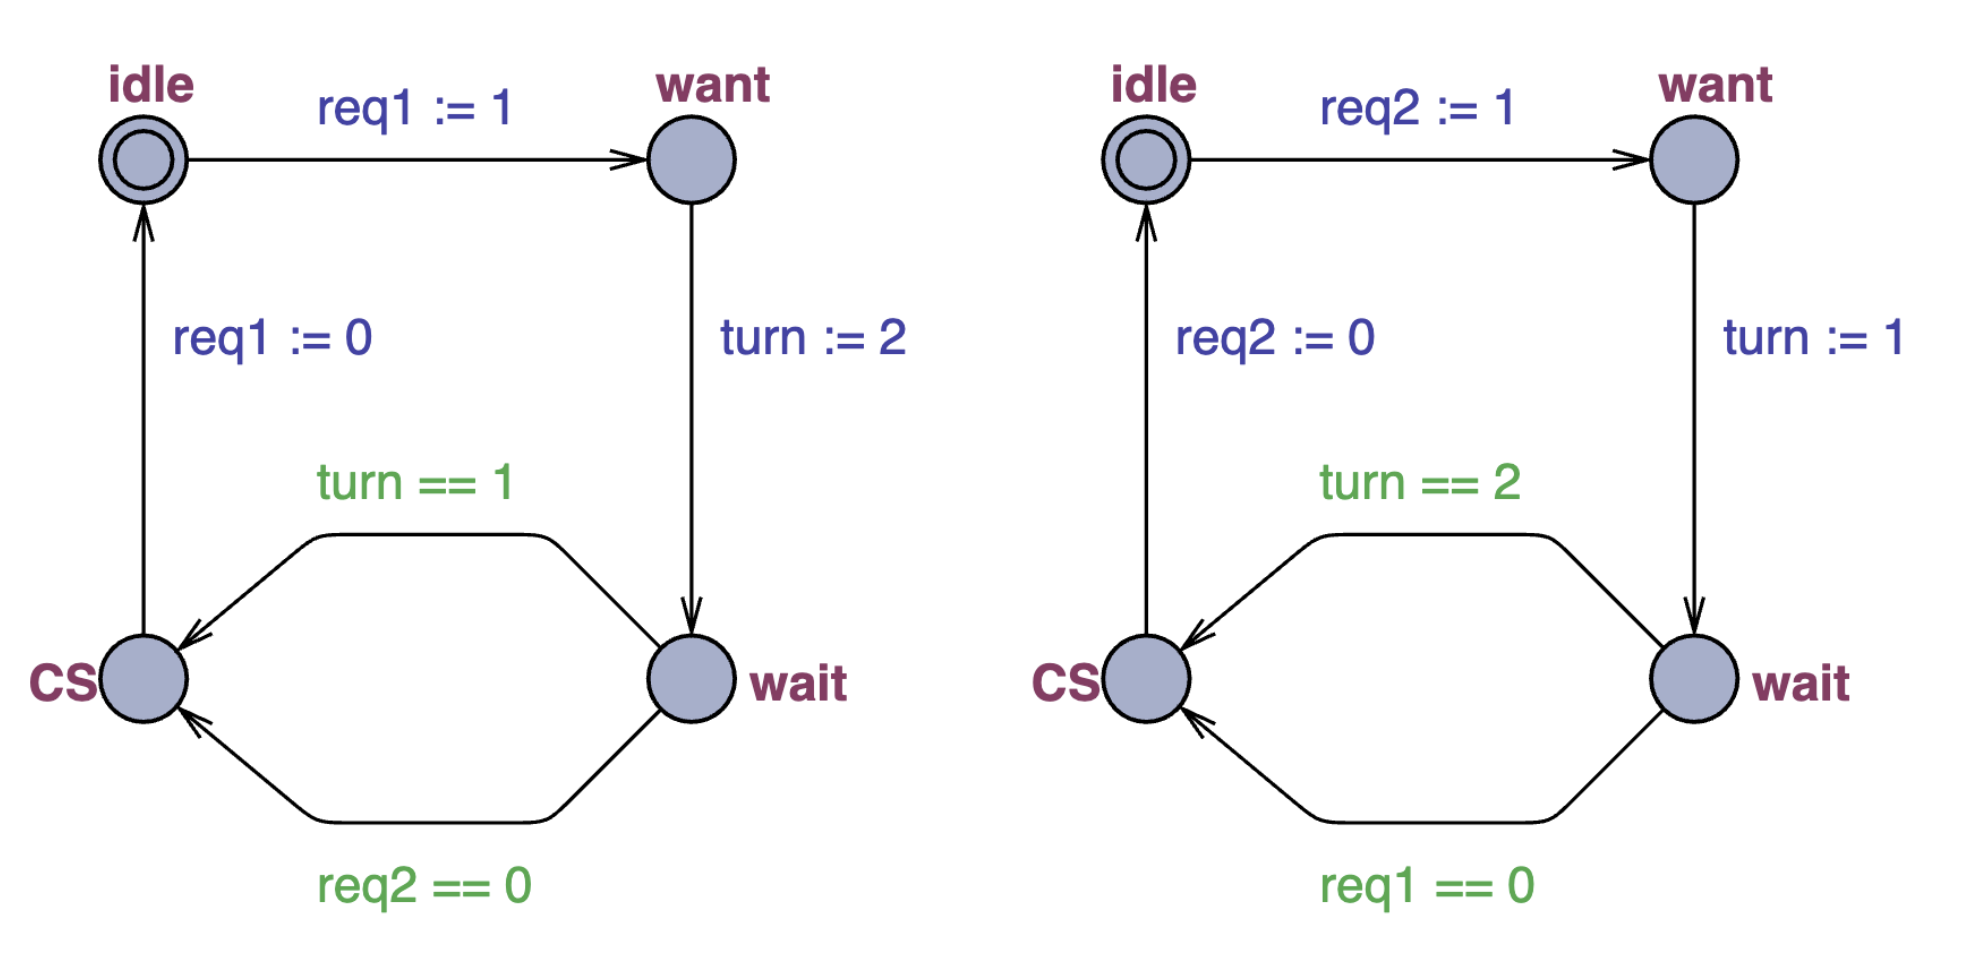
\includegraphics[width=\textwidth]{images/mutex.png}
\label{fig:mutex_uppaal}
\end{figure}



\subsection{Verifying properties in UPPAAL}

% Logical quantifiers in UPPAAL
\begin{definition}[Logical quantifiers in UPPAAL \cite{Bengtsson2004}]
The formulas should be one of the following forms\\
- \texttt{A[]$\phi$} -- Invariantly $\phi$.\\
- \texttt{E<> $\phi$} -- Possibly $\phi$.\\
- \texttt{A<> $\phi$} -- Always Eventually $\phi$.\\
- \texttt{E[] $\phi$} -- Potentially Always $\phi$.\\
- \texttt{$\phi$ --> $\psi$} -- $\phi$ always leads to $\psi$.\\
where $\phi, \psi$ are local properties that can be checked locally on a state, i.e. boolean expressions over predicates on locations and integer variables, and clock constraints.
\label{def:quantifiers}
\end{definition}


% Successfully verified properties for mutex
\begin{figure}[H]
\caption{Successfully verified properties for mutex \cite{SmallTutorial2009}}
\label{fig:mutex_verification}
\begin{lstlisting}[style=code]
A[] not (P1.CS and P2.CS)
E<> P1.CS
E<> P2.CS
\end{lstlisting}    
\end{figure}